\documentclass[11pt,a4paper]{report}

\usepackage[utf8]{inputenc}
\usepackage[T1]{fontenc}
\usepackage[french]{babel}
\usepackage{lmodern}
\usepackage[a4paper,margin=2.5cm]{geometry}
\usepackage{graphicx}
\usepackage{booktabs}
\usepackage{xcolor}
\usepackage{listings}
\usepackage{enumitem}
\usepackage{fancyhdr}
\usepackage{caption}
\usepackage{amsmath}
\usepackage[hidelinks]{hyperref}

\definecolor{accent}{HTML}{4F46E5}
\definecolor{codebg}{HTML}{F6F7FB}
\definecolor{codekw}{HTML}{7C3AED}
\definecolor{codestr}{HTML}{15803D}
\definecolor{codecom}{HTML}{6B7280}

\lstset{
  backgroundcolor=\color{codebg},
  basicstyle=\ttfamily\footnotesize,
  keywordstyle=\color{codekw}\bfseries,
  stringstyle=\color{codestr},
  commentstyle=\color{codecom}\itshape,
  breaklines=true,
  frame=single,
  rulecolor=\color{codebg},
  framesep=6pt,
  xleftmargin=6pt,
  showstringspaces=false,
  columns=fullflexible,
  literate={é}{{\'e}}1 {è}{{\`e}}1 {ê}{{\^e}}1 {à}{{\`a}}1 {â}{{\^a}}1
           {î}{{\^i}}1 {ô}{{\^o}}1 {û}{{\^u}}1 {ù}{{\`u}}1 {ç}{{\c c}}1 {É}{{\'E}}1
}
\lstdefinestyle{ts}{language=Java, morekeywords={const,let,export,interface,type,async,await,function,readonly,return,if,for,of,import,from,number,string,boolean,Date}}

\pagestyle{fancy}
\fancyhf{}
\fancyhead[L]{\small\itshape Planificateur de révisions}
\fancyhead[R]{\small\thepage}
\renewcommand{\headrulewidth}{0.4pt}

\title{%
  \vspace{-1.5cm}
  {\Huge\bfseries Planificateur de révisions}\\[0.4cm]
  {\Large Génération automatique de plannings de révision\\par répétition espacée}\\[1.2cm]
  {\large Rapport technique}
}
\author{Mohamed Aziz Baoueb}
\date{Stage réalisé chez \textbf{Anypli} --- Tunisie\\
Juillet --- Août 2025\\[0.6cm]
\small Refonte complète : octobre 2026}

\begin{document}

\maketitle
\thispagestyle{empty}

\begin{abstract}
\noindent
Ce document décrit la conception et la réalisation d'une application web destinée
aux étudiants : à partir d'une liste d'examens, de leurs coefficients et de la
difficulté des matières concernées, elle produit automatiquement un planning de
révision réparti dans le temps selon le principe de la \emph{répétition espacée}.

Le projet trouve son origine dans un stage d'un mois effectué chez \textbf{Anypli},
en Tunisie, pendant l'été 2025. Je n'avais alors aucune expérience du développement
web : TypeScript, React, Redux et Strapi ont tous été découverts sur place, à
partir de zéro, en quatre semaines. Le présent rapport retrace cet apprentissage,
puis la refonte complète menée ultérieurement, qui a transformé un prototype
fonctionnel en une application structurée, testée et documentée.

Le document assume volontairement un regard critique sur la première version :
en exposer les faiblesses est la manière la plus honnête de mesurer le chemin
parcouru.
\end{abstract}

\tableofcontents

% =====================================================================
\chapter{Contexte}

\section{Le stage chez Anypli}

Ce projet a été réalisé dans le cadre d'un stage d'un mois au sein de l'entreprise
\textbf{Anypli}, en Tunisie, durant l'été 2025. L'objectif du stage était double :
découvrir le développement web moderne dans un cadre professionnel, et livrer une
application complète de bout en bout.

Le point de départ mérite d'être souligné : \textbf{je n'avais aucune connaissance
préalable} des technologies employées. TypeScript, React, la gestion d'état par
Redux, l'architecture d'une API REST, le fonctionnement d'un CMS découplé comme
Strapi --- tout a été appris pendant ces quatre semaines, en même temps que
l'application se construisait. L'historique Git du dépôt en conserve la trace :
les premiers essais datent de la mi-juillet 2025, la version livrée du 15 août 2025.

Apprendre une pile technique entière et produire un livrable dans le même mois
impose des compromis. La première version fonctionnait et répondait au besoin,
mais elle portait les marques de cet apprentissage accéléré. C'est ce constat,
assumé, qui a motivé la refonte décrite au chapitre~\ref{chap:refonte}.

\section{Le besoin}

Un étudiant connaît ses échéances : il sait qu'il a un partiel de mathématiques
dans trois semaines, un oral d'anglais dans dix jours, un projet à rendre dans
un mois. Ce qu'il sait mal faire, c'est \emph{répartir son travail} entre ces
échéances.

Les difficultés sont connues :

\begin{itemize}[nosep]
  \item la tendance à tout réviser la veille, ce que la recherche sur la mémoire
        identifie comme la stratégie la moins efficace ;
  \item la difficulté à pondérer l'effort selon l'importance réelle de chaque
        épreuve ;
  \item l'oubli pur et simple des matières dont l'échéance est lointaine ;
  \item la planification de séances à des moments où l'on n'est, en pratique,
        pas disponible.
\end{itemize}

L'application répond à ce besoin : l'étudiant saisit ses examens et déclare ses
créneaux de disponibilité ; le système produit un planning concret, affiché dans
un calendrier.

\section{Objectifs}

\begin{description}[style=nextline,leftmargin=0.6cm]
  \item[Objectif pédagogique] Maîtriser une pile complète : un langage typé
        (TypeScript), une bibliothèque d'interface (React), une gestion d'état
        (Redux Toolkit) et un backend (Strapi), ainsi que le dialogue entre les
        deux côtés via une API REST.
  \item[Objectif fonctionnel] Livrer une application utilisable : authentification,
        gestion des examens, génération et visualisation d'un planning.
  \item[Objectif de qualité] Atteint lors de la refonte uniquement : rendre le
        projet reproductible, testé et documenté.
\end{description}

% =====================================================================
\chapter{Les technologies découvertes}

Ce chapitre décrit les technologies employées et, pour chacune, ce qu'elle apporte
concrètement au projet.

\section{TypeScript}

TypeScript ajoute un système de types statiques à JavaScript. Son intérêt est de
déplacer la détection des erreurs de l'exécution vers la compilation.

La configuration retenue après refonte active les options les plus strictes :

\begin{lstlisting}[style=ts,caption={Options de compilation, \texttt{tsconfig.json}}]
{
  "strict": true,
  "noUncheckedIndexedAccess": true,
  "exactOptionalPropertyTypes": true,
  "noImplicitOverride": true,
  "noUnusedLocals": true,
  "verbatimModuleSyntax": true
}
\end{lstlisting}

\texttt{noUncheckedIndexedAccess} mérite une mention : il force à traiter
\texttt{tableau[i]} comme potentiellement \texttt{undefined}. C'est contraignant à
l'écriture, mais cela élimine une classe entière d'erreurs à l'exécution.

\section{React}

React construit l'interface à partir de composants : des fonctions qui reçoivent
des données et retournent une description de l'affichage. Le projet utilise React~18
avec les \emph{hooks} (\texttt{useState}, \texttt{useEffect}, \texttt{useMemo}).

\section{Redux Toolkit}

Redux centralise l'état de l'application dans un \emph{store} unique, modifié par
des actions. Redux Toolkit en réduit considérablement la verbosité. Le projet
l'emploie pour l'authentification, la liste des examens, les données de référence
et les notifications.

\section{Strapi}

Strapi est un CMS \emph{headless} : il fournit une base de données, une API REST,
une authentification et une interface d'administration, à partir de la seule
description des types de contenu. C'est ce qui permet, en un mois, de disposer
d'un backend complet sans l'écrire entièrement à la main.

La version~5 introduit le \texttt{documentId}, un identifiant textuel stable qui
remplace l'identifiant numérique dans l'API publique.

\section{Les autres outils}

\begin{table}[h]
\centering
\begin{tabular}{@{}lll@{}}
\toprule
\textbf{Outil} & \textbf{Rôle} & \textbf{Version} \\
\midrule
Vite          & serveur de développement et empaquetage & 5 \\
FullCalendar  & affichage du calendrier                 & 6 \\
i18next       & internationalisation français / anglais & 23 \\
Vitest        & exécution des tests                     & 2 \\
Playwright    & pilotage du navigateur pour la démonstration & 1.49 \\
SQLite        & base de données de développement        & --- \\
PostgreSQL    & base de données de production (Docker)  & 16 \\
\bottomrule
\end{tabular}
\caption{Outils employés}
\end{table}

% =====================================================================
\chapter{La version réalisée pendant le stage}

\section{Ce qui a été livré}

À l'issue du mois, l'application permettait de créer un compte, de se connecter,
de saisir des examens avec une date et un coefficient, de générer un planning de
révision et de le visualiser dans un calendrier. L'interface était traduite en
français et en anglais. Le backend Strapi gérait les relations entre l'utilisateur,
l'élève, les examens et les sessions.

Pour un premier contact avec ces technologies, le résultat était fonctionnel.

\section{Les limites, avec le recul}

Reprendre ce code un an plus tard permet d'en identifier les faiblesses. Les
exposer n'est pas un désaveu : c'est la mesure de ce qui a été appris depuis.

\subsection{Un backend non versionné}

La configuration Strapi --- types de contenu, relations, permissions --- avait été
réalisée à la main dans l'interface d'administration. Elle ne figurait donc nulle
part dans le dépôt. Conséquence directe : \textbf{personne ne pouvait lancer le
projet}. Un clone donnait un écran vide et des erreurs \texttt{403}.

\subsection{Un modèle de données incertain}

Faute de maîtriser le schéma qu'il interrogeait, le code tentait plusieurs noms de
relation jusqu'à ce que l'API cesse de répondre une erreur :

\begin{lstlisting}[style=ts,caption={Extrait de la version~1 --- le code devine son propre modèle}]
const REL_KEYS = ['eleves', 'eleve', 'students'] // essaye plusieurs noms possibles
for (const key of REL_KEYS) {
  try {
    const { data } = await api.get('/api/exams', {
      params: { filters: { [key]: { user: { id: { $eq: userId } } } } }
    })
    fromServer = data?.data ?? []
    break
  } catch (e) { /* mauvais nom : on tente le suivant */ }
}
\end{lstlisting}

\subsection{Un filtrage de sécurité illusoire}

Les examens de \emph{tous} les utilisateurs étaient téléchargés, puis filtrés dans
le navigateur. Le cloisonnement était donc purement cosmétique : n'importe quel
compte authentifié pouvait lire les données des autres en observant les réponses
de l'API.

\subsection{Une erreur de précédence}

La fonction de filtrage contenait un défaut discret :

\begin{lstlisting}[style=ts,caption={Précédence incorrecte entre \texttt{??} et l'opérateur ternaire}]
const eleves =
  a?.eleves?.data ??
  a?.eleve?.data ? [a?.eleve?.data] : []
\end{lstlisting}

La condition évaluée est \texttt{(a?.eleves?.data ?? a?.eleve?.data)}, mais la
valeur retournée est toujours \texttt{[a?.eleve?.data]}. Lorsque la relation
s'appelle \texttt{eleves}, le résultat est \texttt{[undefined]} et le filtrage
échoue en silence.

\subsection{Un algorithme de planification rudimentaire}

Le cœur fonctionnel de l'application tenait en dix-huit lignes :

\begin{lstlisting}[style=ts,caption={Génération du planning, version~1}]
function generatePlan(ex) {
  if (!ex.date || !ex.poids) return []
  const end = new Date(ex.date)
  const nb = Math.max(1, Math.ceil(ex.poids / 10))
  const spanDays = Math.max(3, Math.min(14, nb * 2))
  const sessions = []
  for (let i = nb; i >= 1; i--) {
    const dayOffset = Math.floor((spanDays / (nb + 1)) * i)
    const start = new Date(end)
    start.setDate(end.getDate() - dayOffset)
    start.setHours(18, 0, 0, 0)   // toujours 18 h, toujours 60 minutes
    const fin = new Date(start)
    fin.setMinutes(start.getMinutes() + 60)
    sessions.push({ start, fin })
  }
  return sessions
}
\end{lstlisting}

Cette fonction ignore la date du jour --- elle peut donc produire des séances
\textbf{dans le passé} ---, la difficulté de la matière, les collisions entre
examens et les disponibilités réelles de l'étudiant.

\subsection{Autres points}

\begin{itemize}[nosep]
  \item le type \texttt{any} était omniprésent, ce qui annulait l'intérêt de
        TypeScript ;
  \item les retours à l'utilisateur passaient par \texttt{alert()}, bloquant et
        non testable ;
  \item le dossier \texttt{node\_modules} était versionné, soit 30~Mo inutiles ;
  \item la couverture de test se limitait à un test de fumée.
\end{itemize}

% =====================================================================
\chapter{La refonte}
\label{chap:refonte}

\section{Principes retenus}

\begin{enumerate}[leftmargin=0.8cm]
  \item \textbf{Le projet doit se lancer en deux commandes.} Un projet qu'un tiers
        ne peut pas exécuter n'existe pas.
  \item \textbf{La logique métier doit être isolée.} Le calcul du planning ne
        dépend ni de React ni de Strapi : il est donc testable directement.
  \item \textbf{La configuration est du code.} Schémas et permissions sont
        versionnés, donc reproductibles.
  \item \textbf{La sécurité appartient au serveur.} Aucun filtrage de données
        personnelles n'est délégué au navigateur.
  \item \textbf{Les échecs doivent être explicites.} Une donnée invalide provoque
        une erreur nommée, jamais un résultat silencieusement faux.
\end{enumerate}

\section{Architecture}

\begin{lstlisting}[caption={Organisation du dépôt}]
revision-planner/
|-- packages/core/   Moteur de planification -- TypeScript pur, 32 tests
|-- apps/api/        Backend Strapi 5 -- schemas, permissions, donnees de demo
|-- apps/web/        Frontend React 18 + Vite + Redux Toolkit, 13 tests
`-- scripts/         Capture automatisee de la demonstration
\end{lstlisting}

Le choix d'un \emph{monorepo} permet au front et au moteur de partager exactement
les mêmes types, sans duplication ni publication de paquet intermédiaire.

\section{Modèle de données}

\begin{table}[h]
\centering
\begin{tabular}{@{}lp{9.5cm}@{}}
\toprule
\textbf{Type} & \textbf{Rôle} \\
\midrule
\texttt{student} & Profil étudiant, rattaché à un compte utilisateur, porteur des disponibilités et des préférences de durée \\
\texttt{subject} & Matière et sa difficulté (\emph{facile}, \emph{moyen}, \emph{difficile}) \\
\texttt{exam}    & Épreuve : intitulé, date, coefficient, type, matière, élève \\
\texttt{revision-session} & Créneau de révision généré, rattaché à un examen \\
\bottomrule
\end{tabular}
\caption{Types de contenu}
\end{table}

Les noms sont désormais fixés et versionnés dans \texttt{apps/api/src/api/*/con\-tent-types/}.
Il n'y a plus rien à deviner à l'exécution.

% =====================================================================
\chapter{Le moteur de planification}

C'est la pièce centrale du projet. Elle est implémentée dans
\texttt{packages/core} sous forme de fonctions pures, sans dépendance externe.

\section{Volume de révision}

Le temps accordé à un examen dépend de son coefficient et de la difficulté de sa
matière :

\begin{equation}
  M = \left\lceil \frac{c \times 6 \times f_d}{s} \right\rceil \times s
\end{equation}

où $c$ est le coefficient, $f_d$ le facteur de difficulté
($0{,}75$ \emph{facile}, $1$ \emph{moyen}, $1{,}35$ \emph{difficile}), $s$ la durée
d'une séance en minutes, et $M$ le volume total accordé. L'arrondi au multiple
supérieur de $s$ traduit un choix explicite : on ne planifie pas une fraction de
séance.

\begin{table}[h]
\centering
\begin{tabular}{@{}lccc@{}}
\toprule
\textbf{Examen} & \textbf{Coefficient} & \textbf{Difficulté} & \textbf{Séances} \\
\midrule
Anglais technique    & 10 & facile    & 1 \\
Modélisation SQL     & 20 & moyen     & 2 \\
Protocoles réseau    & 30 & moyen     & 3 \\
Mécanique quantique  & 35 & difficile & 5 \\
Analyse numérique    & 40 & difficile & 6 \\
\bottomrule
\end{tabular}
\caption{Répartition obtenue sur le jeu de données de démonstration}
\end{table}

\section{Répétition espacée}

Les séances sont placées à des intervalles croissants avant l'épreuve. Les écarts
successifs valent $1, 2, 3, 4, \ldots$ jours, ce qui donne les décalages cumulés :

\begin{equation}
  d_k = \sum_{i=1}^{k} i = \frac{k(k+1)}{2}
  \qquad \text{soit } 1,\ 3,\ 6,\ 10,\ 15,\ 21,\ \ldots
\end{equation}

La révision est ainsi dense à l'approche de l'examen et de plus en plus espacée en
remontant dans le temps, conformément au principe de la répétition espacée, qui
favorise la mémorisation durable.

\subsection{Adaptation à la fenêtre disponible}

Pour dix séances, le décalage le plus lointain vaut $d_{10} = 55$ jours. Si
l'examen a lieu dans vingt jours, viser ces dates condamne la moitié des séances.
Les décalages sont donc comprimés proportionnellement :

\begin{equation}
  d'_k = \operatorname{round}\left(d_k \times \frac{L}{d_n}\right)
  \quad \text{lorsque } d_n > L
\end{equation}

où $L$ est le nombre de jours réellement disponibles. L'ordre et la progression
des écarts sont conservés.

Ce point est le résultat direct d'une relecture critique : la première
implémentation du moteur perdait trois séances sur dix dans ce cas de figure et
les imputait, à tort, à un manque de créneaux.

\section{Placement des séances}

Pour chaque séance, l'algorithme procède ainsi :

\begin{enumerate}[nosep,leftmargin=0.8cm]
  \item calculer la date idéale, soit la date de l'examen moins le décalage ;
  \item explorer les journées autour de cette date, en privilégiant d'abord la
        date exacte puis les jours antérieurs ;
  \item pour chaque journée, parcourir les créneaux de disponibilité et y chercher
        un intervalle libre, en respectant les pauses et le plafond journalier ;
  \item en dernier recours, balayer toute la fenêtre restante plutôt que
        d'abandonner la séance.
\end{enumerate}

Les examens sont traités du plus proche au plus lointain : en cas de pénurie de
créneaux, ce sont les échéances lointaines qui cèdent.

\section{Garanties}

Le moteur garantit, et ses tests le vérifient :

\begin{itemize}[nosep]
  \item aucune séance dans le passé, ni après la date de l'examen concerné ;
  \item une marge de repos configurable avant chaque épreuve ;
  \item aucun chevauchement entre deux séances, y compris pour des examens
        différents ;
  \item le respect des créneaux, des pauses et du plafond journalier ;
  \item un résultat déterministe à données identiques.
\end{itemize}

\section{Diagnostics}

Lorsqu'une séance ne peut pas être placée, le moteur ne l'omet pas en silence : il
renvoie une cause explicite --- \emph{examen déjà passé}, \emph{aucune
disponibilité}, ou \emph{temps insuffisant} --- affichée à l'utilisateur avant
l'enregistrement.

\section{Validation des entrées}

Un coefficient non fini provoque une erreur nommée plutôt qu'un résultat aberrant :

\begin{lstlisting}[style=ts]
if (!Number.isFinite(exam.weight)) {
  throw new RangeError(
    `Coefficient invalide pour "${exam.name}" : ${exam.weight}`)
}
\end{lstlisting}

Cette vérification est née d'une revue : sans elle, un coefficient \texttt{NaN}
faisait disparaître l'examen du planning sans le moindre avertissement --- le
défaut même reproché à la version~1.

% =====================================================================
\chapter{Le backend}

\section{Permissions appliquées par le code}

Les permissions du rôle \emph{authenticated} sont posées au démarrage, et non
cochées à la main dans l'administration :

\begin{lstlisting}[style=ts,caption={\texttt{src/bootstrap/permissions.ts}, extrait}]
const AUTHENTICATED_ACTIONS = [
  'api::exam.exam.find', 'api::exam.exam.create',
  'api::exam.exam.update', 'api::exam.exam.delete',
  'api::revision-session.revision-session.find',
  /* ... */
]
\end{lstlisting}

L'opération est idempotente. Sur une base vierge, le démarrage applique quinze
permissions authentifiées et une publique, puis injecte les données de
démonstration. C'est ce qui rend l'installation reproductible et supprime les
erreurs \texttt{403} de la version~1.

\section{Cloisonnement des données}

Chaque requête est filtrée côté serveur par le profil étudiant du compte appelant :

\begin{lstlisting}[style=ts,caption={Contrôleur \texttt{exam}, méthode \texttt{find}}]
async find(ctx) {
  const student = await requireStudent(strapi, ctx)
  ctx.query = {
    ...ctx.query,
    filters: {
      ...ctx.query?.['filters'],
      student: { documentId: { $eq: student.documentId } },
    },
  }
  return super.find(ctx)
}
\end{lstlisting}

En écriture, la relation \texttt{student} est imposée par le serveur : un examen ne
peut pas être créé pour autrui, ni réaffecté. Une requête sans jeton reçoit un
\texttt{403}.

\section{Données de démonstration}

Le jeu de démonstration emploie des dates \emph{relatives} au jour du démarrage.
La démonstration reste donc pertinente quelle que soit la date à laquelle le dépôt
est cloné, au lieu d'afficher des examens périmés.

% =====================================================================
\chapter{L'interface}

\begin{figure}[h]
\centering
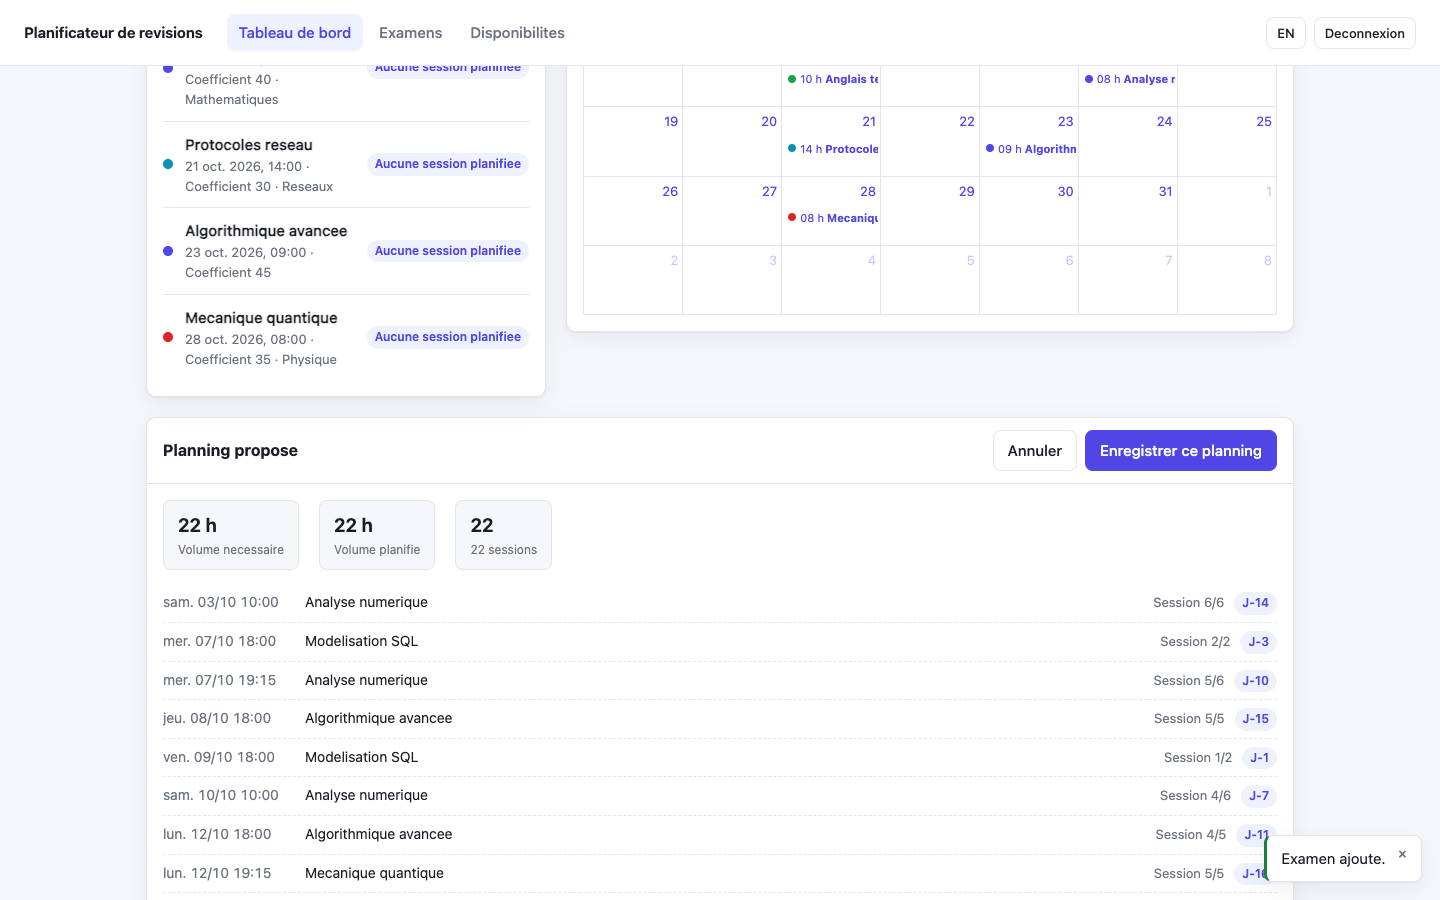
\includegraphics[width=\textwidth]{../media/frames/0007-planning-previsualisation.png}
\caption{Prévisualisation du planning avant enregistrement : volume nécessaire,
volume planifié, et chaque séance datée avec son rang et son écart à l'examen.}
\end{figure}

\section{Prévisualisation avant enregistrement}

La version~1 écrivait directement en base puis affichait
\texttt{alert('Plan généré')}. L'étudiant ne voyait ni ce qui avait été créé, ni
les échecs partiels. La refonte introduit une étape de prévisualisation : le
planning est calculé, présenté avec ses diagnostics, et n'est enregistré
qu'après confirmation.

\section{Déclaration des disponibilités}

\begin{figure}[h]
\centering
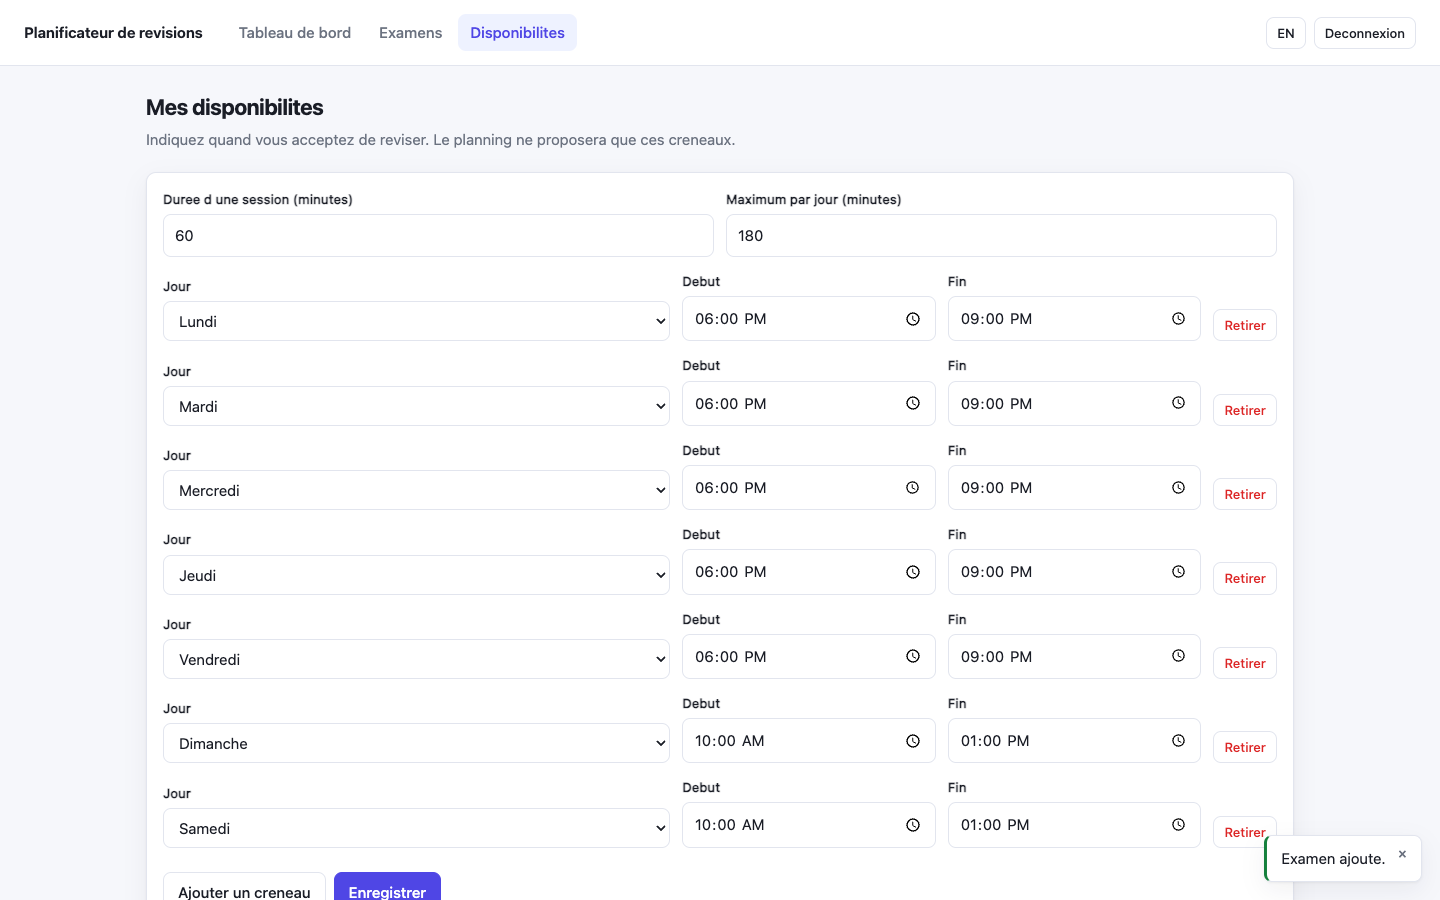
\includegraphics[width=\textwidth]{../media/frames/0006-disponibilites.png}
\caption{Édition des créneaux hebdomadaires. Le planning ne propose que ces plages.}
\end{figure}

Cette page n'existait pas auparavant : les séances étaient systématiquement placées
à 18~h pour une heure, sans jamais demander son avis à l'étudiant.

\section{Notifications}

Les \texttt{alert()} ont été remplacés par une pile de notifications non
bloquantes, gérée dans le \emph{store} Redux. Outre le confort, ce choix rend
l'interface vérifiable automatiquement : un \texttt{alert()} suspend le navigateur
et interrompt tout pilotage par Playwright.

% =====================================================================
\chapter{Qualité}

\section{Tests}

\begin{table}[h]
\centering
\begin{tabular}{@{}lcp{7cm}@{}}
\toprule
\textbf{Paquet} & \textbf{Tests} & \textbf{Portée} \\
\midrule
\texttt{packages/core} & 32 & volume, espacement, garanties, cas limites, validation des entrées \\
\texttt{apps/web}      & 13 & sérialiseur de requêtes, parité des traductions, conversion des données \\
\midrule
\textbf{Total}         & \textbf{45} & \\
\bottomrule
\end{tabular}
\caption{Couverture de test}
\end{table}

Un enseignement de la relecture mérite d'être noté : les premiers tests écrits
validaient surtout mes propres hypothèses. Ce sont les tests portant sur les
\emph{cas limites} --- coefficient invalide, fenêtre trop courte, calendrier
saturé --- qui ont révélé les véritables défauts.

\section{Démonstration reproductible}

Le script \texttt{scripts/capture-demo.mjs} pilote l'application avec Playwright,
enregistre une image à chaque étape, puis assemble une vidéo et un GIF avec ffmpeg.
Il réinitialise les données avant de filmer, ce qui le rend rejouable à
l'identique. La démonstration se régénère donc après chaque évolution de
l'interface, au lieu d'être un enregistrement manuel vite périmé.

% =====================================================================
\chapter{Difficultés rencontrées}

\section{Pendant le stage}

La difficulté principale fut le volume de notions à acquérir simultanément :
typage statique, programmation par composants, gestion d'état centralisée,
protocole REST, relations entre types de contenu, authentification par jeton.
Chaque obstacle technique se doublait d'un obstacle conceptuel.

Le dialogue entre le front et Strapi fut le point le plus coûteux, en particulier
la structure des réponses, les relations à peupler explicitement, et la
configuration des permissions --- dont la méconnaissance explique les
contournements relevés au chapitre~3.

\section{Pendant la refonte}

\begin{description}[style=nextline,leftmargin=0.6cm]
  \item[Un cache de paquets corrompu] Une installation interrompue avait laissé
        des paquets incomplets. Trois pannes sans rapport apparent en découlaient :
        \texttt{ts.sys undefined}, une erreur de schéma \texttt{yup}, et un build
        Strapi impossible. Une réinstallation propre les a toutes résolues d'un
        coup. Leçon : remonter à la cause commune plutôt que traiter les symptômes.
  \item[Une variable d'environnement vide] \texttt{DATABASE\_FILENAME=} renvoyait
        une chaîne vide plutôt que la valeur par défaut ; Strapi tentait alors
        d'ouvrir un \emph{répertoire} comme base de données.
  \item[Un dossier synchronisé] Le projet résidait initialement sur un Bureau
        synchronisé par iCloud Drive. Les démons de synchronisation génèrent des
        événements système que les observateurs de fichiers de Vite et de Strapi
        interprètent comme des modifications, provoquant des redémarrages en
        boucle. Un projet Node n'a pas sa place dans un dossier synchronisé.
\end{description}

% =====================================================================
\chapter{Bilan et perspectives}

\section{Ce que le stage a apporté}

En un mois chez Anypli, je suis passé d'une absence totale d'expérience en
développement web à une application complète et fonctionnelle : interface React
typée, backend Strapi, authentification, internationalisation, affichage
calendaire. Cet apprentissage accéléré constitue le véritable acquis du stage, et
la première version doit être jugée à cette aune.

\section{Ce que la refonte a apporté}

La refonte relève d'une autre compétence : non plus faire fonctionner, mais rendre
\emph{fiable}. Isoler la logique métier pour la tester, versionner la
configuration pour la rendre reproductible, placer la sécurité au bon endroit,
rendre les échecs explicites --- autant de réflexes qui ne s'acquièrent qu'en
reprenant son propre code avec du recul.

\begin{table}[h]
\centering
\begin{tabular}{@{}lll@{}}
\toprule
 & \textbf{Version 1} & \textbf{Version 2} \\
\midrule
Backend          & à configurer à la main      & versionné dans le dépôt \\
Lancement        & impossible sans réglages    & \texttt{npm install \&\& npm run dev} \\
Planification    & 18 lignes                   & moteur isolé et testé \\
Séances passées  & générées                    & impossibles par construction \\
Filtrage         & navigateur                  & serveur \\
Tests            & 1                           & 45 \\
TypeScript       & \texttt{any} omniprésent    & strict, sans \texttt{any} \\
\bottomrule
\end{tabular}
\caption{Comparaison des deux versions}
\end{table}

\section{Perspectives}

\begin{itemize}[nosep]
  \item ajuster les constantes du moteur --- six minutes par point de coefficient
        et les facteurs de difficulté sont des choix de conception, non des
        valeurs établies ; les rendre configurables par l'étudiant serait un
        progrès ;
  \item gérer explicitement les fuseaux horaires, aujourd'hui alignés sur celui du
        navigateur ;
  \item tenir compte de l'avancement réel des séances pour replanifier ce qui n'a
        pas été fait ;
  \item exporter le planning au format iCalendar.
\end{itemize}

\vfill
\begin{center}
\small
Code source : \url{https://github.com/aziz3r/revision-planner}
\end{center}

\end{document}
